\documentclass[xcolor=dvipsnames]{beamer}
\usecolortheme[named=MidnightBlue]{structure}
\definecolor{blue(ryb)}{rgb}{0.2, 0.2, 0.6}
\definecolor{blue(ryb)}{rgb}{0.01, 0.28, 1.0}
\definecolor{bostonuniversityred}{rgb}{0.8, 0.0, 0.0}
\DeclareGraphicsExtensions{jpg,eps,png}
 \renewcommand{\thefootnote}{\fnsymbol{footnote}}
\usetheme{Boadilla} 
%--------------modify footer
\makeatother
\setbeamertemplate{footline}
{
  \leavevmode%
  \hbox{%
   \begin{beamercolorbox}[wd=.4\paperwidth,ht=2.25ex,dp=1ex,center]{section in head/foot}%
    \usebeamerfont{section in head/foot}\insertsectionhead
  \end{beamercolorbox}%
  \begin{beamercolorbox}[wd=.6\paperwidth,ht=2.25ex,dp=1ex,center]{title in head/foot}%
    \usebeamerfont{section in head/foot}\insertshorttitle\hspace*{3em}
    \insertframenumber{} / \inserttotalframenumber\hspace*{1ex}
  \end{beamercolorbox}}%
  \vskip0pt%
}
\makeatletter
\setbeamertemplate{navigation symbols}{}
%---------------------------modify footer end
%\hypersetup{pdfpagemode=FullScreen}
\usepackage{epsfig}
\usepackage{graphicx}
\usepackage{epstopdf}
%-------------------------------------
%Title
%-------------------------------------

\title[]{Communication Efficient Data Exchange Among Multiple Nodes}
\author[]{Soumya Subhra Banerjee,  }
\normalsize
\institute[ECE, IISc]{Project presentation, E2 207 -- Concentration Inequalities\footnote[2]{ \tiny \textit{presented by} K. R. Sahasranand, Dept. of Electrical Communication Engg., IISc.}}
\date{\today}
%====================================Title
\begin{document}
\begin{frame}
\titlepage
\end{frame}
%====================================Overview

\section{Introduction}
\begin{frame}
\frametitle{Proof Outline}
\begin{itemize}
\item Preliminaries
\item Key ingredients
\begin{itemize}
\item Reed Muller codes are doubly transitive
\item {\color{blue(ryb)}Symmetric monotone sets have sharp thresholds}
\item EXIT\footnote[2]{EXtrinsic Information Transfer} functions satisfy the area theorem
\end{itemize}
\item Conclusion
\end{itemize}
\end{frame}

\begin{frame}
\frametitle{Preliminaries}
\framesubtitle{Binary Erasure Channel (BEC) and MAP decoder}
\begin{figure}[!htb]
\begin{center}
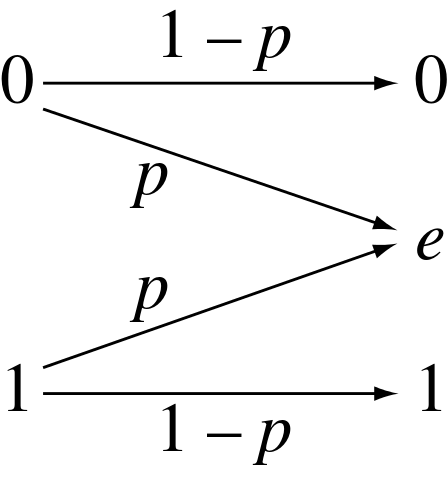
\includegraphics[scale=0.18]{./figures/bec.png}
\caption{Denoted BEC($p$). If $X_i$ is transmitted over BEC($p_i$), referred to as BEC($\underline{p}$)}
\label{fig:bec}
\end{center}
\end{figure}
\begin{itemize}
\item $D_i : \mathcal{Y}^N \to \mathcal{X} \cup \{e\}$ : bit-MAP decoder for bit $i$.
\item Erasure probability for bit $i \in [N]$, $P_{b,i} \triangleq \mathbb{P}[D_i(\underline{Y}) \neq X_i]$. \\
Average bit erasure probability, $P_b \triangleq \frac{1}{N}\sum_{i=1}^N P_{b,i}$.
\item If bit $i$ is recovered given $\underline{y}$, $H(X_i|\underline{Y}=\underline{y}) = 0$. \\Otherwise, uniform codeword assumption $\Rightarrow H(X_i|\underline{Y}=\underline{y}) = 1$. Thus, $P_{b,i} = H(X_i|\underline{Y}) \text{ and, } P_b = \frac{1}{N}\sum_{i=1}^N  H(X_i|\underline{Y}).$
\end{itemize}
\end{frame}

\begin{frame}
\frametitle{Preliminaries}
\framesubtitle{MAP EXIT functions}
The vector EXIT function associated with bit $i$ of the (uniformly randomly chosen) codeword $$h_i(\underline{p})\triangleq H(X_i | \underline{Y}_{-i}(\underline{p}_{-i})).$$ The average vector EXIT function is defined by $$h(\underline{p}) \triangleq \frac{1}{N}\sum_{i=1}^N h_i(\underline{p}).$$ Scalar EXIT functions defined by choosing $\underline{p}=(p,p,\ldots,p)$.
\begin{align*}
H(X_i|\underline{Y}) &= \mathbb{P}(Y_i=e)H(X_i|\underline{Y}_{-i}, Y_i=e) + \mathbb{P}(X_i=Y_i)H(X_i|\underline{Y}_{-i}, Y_i=X_i)\\
&= \mathbb{P}(Y_i=e)H(X_i|\underline{Y}_{-i}).
\end{align*}
Therefore, $P_{b,i}(p) = ph_i(p)$ and $P_b(p) = ph(p)$ \hspace{2cm}$(3)$
\end{frame}

\begin{frame}
\frametitle{Preliminaries}
\framesubtitle{More definitions}
\emph{Definition $2$} - Consider a code $\mathcal{C}$ and the \emph{indirect recovery} of $X_i$ from the subvector $\underline{Y}_{-i}$ (i.e., the bit-MAP decoding of $Y_i$ from $\underline{Y}$ when $Y_i=e$). For $i \in [N]$, the set of erasure patterns that prevent indirect recovery of $X_i$ under bit-MAP decoding is given by $$\Omega_i \triangleq \{A \subseteq [N]\backslash\{i\} : \exists B \subseteq [N]\backslash\{i\}, B \cup \{i\} \in \mathcal{C}, B \subseteq A\}.$$ For distinct $i,j \in [N]$, the set of erasure patterns where the $j$-th bit is \emph{pivotal} for the indirect recovery of $X_i$ is given by $$\partial_j\Omega_i \triangleq \{A \subseteq [N]\backslash\{i\}: A\backslash \{j\} \notin \Omega_i, A \cup \{j\} \in \Omega_i \}$$ These are the erasure patterns where $X_i$ can be recovered from $\underline{Y}_{-i}$ iff $Y_j \neq e$.
\end{frame}

\begin{frame}
\begin{block}{Proposition $4$}
For a code $\mathcal{C}$ and transmission over a BEC, we have the following properties for the EXIT functions.
\begin{enumerate}
\item[(a)] The EXIT function associated with bit $i$ satisfies $$h_i(p) = \sum_{A \in \Omega_i} p^{|A|}(1-p)^{N-1-|A|}.$$
\item[(b)] For $j \in [N]\backslash\{i\}$, the partial derivative satisfies $$\frac{\partial h_i(\underline{p})}{\partial p_j}\Bigg|_{\underline{p}=(p,p,\ldots,p)} = \sum_{A \in \partial_j\Omega_i} p^{|A|}(1-p)^{N-1-|A|}.$$
\item[(c)]The average EXIT function satisfies the \emph{area theorem} $$\int_0^1 h(p)dp = \frac{K}{N}.$$
\end{enumerate}
\end{block}
\end{frame}

\begin{frame}
\frametitle{Preliminaries}
\framesubtitle{Permutations of linear codes}
$S_N$, the symmetric group on $N$ elements. The permutation group of a code is defined as the subgroup of $S_N$ whose group action on the bit ordering preserves the set of codewords.\\
\vspace{1cm}
\emph{Definition $5$} - The permutation group $\mathcal{G}$ of a code $\mathcal{C}$ is defined to be $$\mathcal{G} = \{\pi \in S_N : \pi(A) \in \mathcal{C} \text{ for all } A \in \mathcal{C}\}.$$\\
\emph{Definition $6$} - Suppose $\mathcal{G}$ is a permutation group. Then,
\begin{enumerate}
\item[(a)]$\mathcal{G}$ is \emph{transitive} if, for any $i,j \in [N]$, there exists a permutation $\pi \in \mathcal{G}$ such that $\pi(i)=j$, and
\item[(b)] $\mathcal{G}$ is \emph{doubly transitive} if, for any distinct $i,j,k \in [N]$, there exists a $\pi \in \mathcal{G}$ such that $\pi(i)=i$ and $\pi(j)=k$.
\end{enumerate}
\end{frame}

\begin{frame}
\frametitle{}
\begin{block}{Proposition $7$}
Suppose the permutation group $\mathcal{G}$ of a code $\mathcal{C}$ is transitive. Then, for any $i \in [N]$, $$h(p) = h_i(p) \text{ for } 0 \le p\le 1.$$
\end{block}
\begin{block}{Proposition $8$}
Suppose the permutation group $\mathcal{G}$ of a code $\mathcal{C}$ is doubly transitive. Then, for distinct $i,j,k \in [N]$, and any $0 \le p \le 1$, $$\frac{\partial h_i(\underline{p})}{\partial p_j'}\Bigg|_{\underline{p}=(p,p,\ldots,p)} = \frac{\partial h_i(\underline{p})}{\partial p_k'}\Bigg|_{\underline{p}=(p,p,\ldots,p)}.$$

\end{block}
\end{frame}

\begin{frame}
\frametitle{Capacity achieving codes and the EXIT function}
\emph{Definition} : Suppose $\{\mathcal{C}_n\}$ is a sequence of codes with rates $\{r_n\}$ where $r_n \to r$ for $r \in (0,1)$. $\{\mathcal{C}_n\}$ is said to be {\color{blue(ryb)}capacity achieving} on the BEC under bit-MAP decoding, if for any $p \in [0, 1-r)$, the average bit-erasure probabilities satisfy $$\lim_{n \to \infty} P_b^{(n)}(p) = 0.$$
\begin{figure}[!htb]
\begin{center}
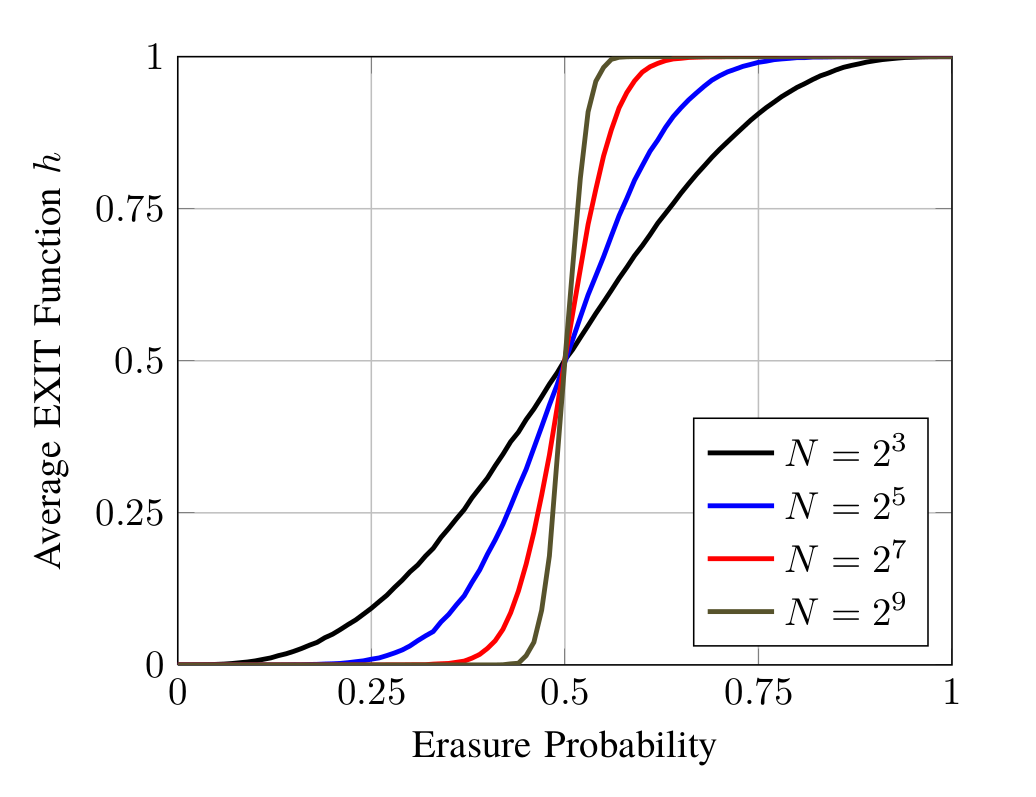
\includegraphics[scale=0.18]{./figures/exitfun.png}
\label{fig:exitfun}
\end{center}
\end{figure}
\end{frame}

\begin{frame}
\begin{block}{Proposition $10$}
Let $\{\mathcal{C}_n\}$ be a seq. of codes with rates $\{r_n\}$, $r_n \to r$ for $r \in (0,1)$. TFAE - 
\begin{enumerate}
\item[S1:] $\{\mathcal{C}_n\}$ is capacity achieving on the BEC under bit-MAP decoding.
\item[S2:] The sequence of average EXIT functions satisfies
\[
    \lim_{n \to \infty} h^{(n)}(p)=\left\{
                \begin{array}{ll}
                  0 \text{ if } 0 \le p < 1-r\\
                  1 \text{ if } 1-r < p \le 1.\\
                \end{array}
              \right.
  \]
\item[S3:] For any $0 < \epsilon \le 1/2$, $$\lim_{n \to \infty} p_{1-\epsilon}^{(n)} - p_{\epsilon}^{(n)} = 0.$$
\end{enumerate}
\end{block}
\emph{Proof}: 
\begin{itemize}
\item S2 $\Rightarrow$ S1 : $P_b(p) = ph(p)$.
\item S1 $\Rightarrow$ S2 : $P_b(p) = ph(p)$ and \emph{Area Theorem} (Proposition $4$).
\item S2 $\Rightarrow$ S3 : $p_{1-\epsilon}^{(n)} - p_{\epsilon}^{(n)}$  $\sim$ $h^{(n)}$ transitions from $\epsilon$ to $1-\epsilon$.
\item S3 $\Rightarrow$ S2 :  Suffices to show, $\lim_{n \to \infty} p_\epsilon^{(n)} = \lim_{n \to \infty} p_{1-\epsilon}^{(n)} = 1-r$. \\
$\hspace{1.84cm}$Use Area Theorem.
\end{itemize}
\end{frame}

\begin{frame}
\frametitle{More definitions}
Define 
\[
    [\phi_i(A)]=\left\{
                \begin{array}{ll}
                  \mathbf{1}_A(l) \text{ if } l < i\\
                  \mathbf{1}_A(l+1) \text{ if } l \ge i.\\
                \end{array}
              \right.
  \]
Now define
\begin{align*}
\Omega_i' &\triangleq \{\phi_i(A) \in \{0,1\}^{N-1} : A \in \Omega_i\}\\
\partial_j\Omega_i' &\triangleq \{\phi_i(A) \in \{0,1\}^{N-1}: A \in \partial_j\Omega_i\}. &&(8)
\end{align*}
Consider the space $\{0,1\}^M$ with a measure $\mu_p$ such that $$\mu_p(\Omega) = \sum_{\underline{x} \in \Omega} p^{|\underline{x}|}(1-p)^{M-|\underline{x}|}, \text{ for }\Omega \subseteq \{0,1\}^M,$$ where the weight $|\underline{x}| = x_1 + x_2 + \ldots + x_M$ is the number of $1$'s in $\underline{x}$. \\Using proposition $4$, $h_i(p)=\mu_p(\Omega_i')$ with $M=N-1$.
\end{frame}

\begin{frame}
\frametitle{Invoking something we learnt..}
\begin{block}{Theorem $16$}
Let $\Omega$ be a monotone set and suppose that, for all $0 \le p \le 1$, the influences of all bits are equal $I_1^{(p)}(\Omega) = \ldots = I_M^{(p)}(\Omega)$. Then, for any $0 < \epsilon \le 1/2$, $$p_{1-\epsilon} - p_\epsilon \le \frac{2 \log \frac{1-\epsilon}{\epsilon}}{C\log (N-1)},$$ where $p_t = \inf\{p \in [0,1] : \mu_p (\Omega) \ge t\}$ is well defined because $\mu_p(\Omega)$ is strictly increasing in $p$ with $\mu_0(\Omega) = 0$ and $\mu_1(\Omega)=1$.
\end{block}
\emph{Proof}: Using Russo's lemma.
\end{frame}


\begin{frame}
\frametitle{... and finally ~~~~~~~~~~~~~\tiny{Wake up folks! It's the main result :)}}
\begin{block}{Theorem $17$}
Let $\{\mathcal{C}_n\}$ be a sequence of codes where the blocklengths satisfy $N_n \to \infty$, the rates satisfy $r_n \to r$, and the permutation group $\mathcal{G}(n)$ (of $\mathcal{C}_n$) is doubly transitive for each $n$. If $r \in (0,1)$, then $\{\mathcal{C}_n\}$ is capacity achieving on the BEC under bit-MAP decoding.
\end{block}
\normalsize
\emph{Proof}: \\Let the average EXIT function of $\mathcal{C}_n$ be $h^{(n)}$. Fix some $i \in [N]$. Since $\mathcal{G}$ is transitive, from Proposition $7$, $$h(p) = h_i(p) \text{ for all } p \in [0,1].$$

Consider the sets $\Omega_i'$ from Definition $2$ and Equation $(8)$, and let $M=N-1$. 
\end{frame}

\begin{frame}
\frametitle{Proof of Theorem $17$ (contd.)}
Observe that, from Proposition $4$,
\begin{align*}
h_i(p) = \mu_p(\Omega_i'), &&I_j^{p}(\Omega_i') = \frac{\partial h_i(\underline{p})}{\partial p_j'}\Bigg|_{\underline{p}=(p,p,\ldots,p)}
\end{align*}
where $j'$ is given by 
\[
    j'=\left\{
                \begin{array}{ll}
                  j \text{ if } j < i\\
                  j+1 \text{ if } j \ge i.\\
                \end{array}
              \right.
  \]
Since $\mathcal{G}$ is doubly transitive, from Proposition $8$, $$I_j^{p}(\Omega_i') = I_k^{p}(\Omega_i') \text{ for all } j,k \in [N-1].$$
\end{frame}

\begin{frame}
\frametitle{Proof of Theorem $17$ (contd.)}
Using Theorem $16$, we have $$p_{1-\epsilon} - p_\epsilon \le \frac{2 \log \frac{1-\epsilon}{\epsilon}}{C\log (N-1)},$$ where $p_t$ is the functional inverse of $h$ as in Theorem $16$. Since $N \to \infty$ from the hypothesis, $$\lim_{n \to \infty} (p_{1-\epsilon} - p_\epsilon) = 0.$$

Now, using Proposition $10$, $\{\mathcal{C}_n\}$ is capacity achieving on the BEC under bit-MAP decoding. \\$\square$
\end{frame}

\begin{frame}{References}
\begin{enumerate}
\item[(1)] S. Kumar and H. D. Pfister, “Reed-Muller codes achieve
capacity on erasure channels,” 2015, [Online]. Available:
http://arxiv.org/abs/1505.05123v2.
\item[(2)] S. Kudekar, M. Mondelli, E. \c{S}a\c{s}\u{o}glu, and R. Urbanke, “Reed-Muller codes achieve capacity on the binary erasure channel under MAP
decoding,” 2015, [Online]. Available: http://arxiv.org/abs/1505.05831v1.
\item[(3)] {\color{MidnightBlue}$\equiv (1) \cup (2)$} S. Kudekar, S. Kumar, M. Mondelli, H. D. Pfister, E. \c{S}a\c{s}\u{o}glu, and R. Urbanke, “Reed-Muller codes achieve
capacity on erasure channels,” 2016, [Online]. Available:
http://arxiv.org/abs/1601.04689v1.
\end{enumerate}
\end{frame}

\begin{frame}
\frametitle{}
\begin{figure}[!htb]
\begin{center}

\includegraphics[scale=0.35]{./figures/questions.jpg}
\end{center}
\end{figure}
\begin{block}{}
\centering
Thank You!
\end{block}
\end{frame}

\end{document}